\documentclass[a4paper,10pt]{article}
\usepackage[utf8x]{inputenc}
\usepackage[slovene]{babel}
\usepackage{amsmath}
\usepackage{amsfonts}
\usepackage{relsize}
\usepackage[smaller]{acronym}
\usepackage{graphicx}
\usepackage{subfigure}
\usepackage{cite}
\usepackage{url}
\usepackage{hyperref}

\renewcommand{\theta}{\vartheta}
\renewcommand{\phi}{\varphi}

\newcommand{\dd}{\,\mathrm{d}}

\title{Fourierova analiza}
\author{Miha \v Can\v cula}

\begin{document}
  \maketitle

\begin{figure}[h]
  \centering
  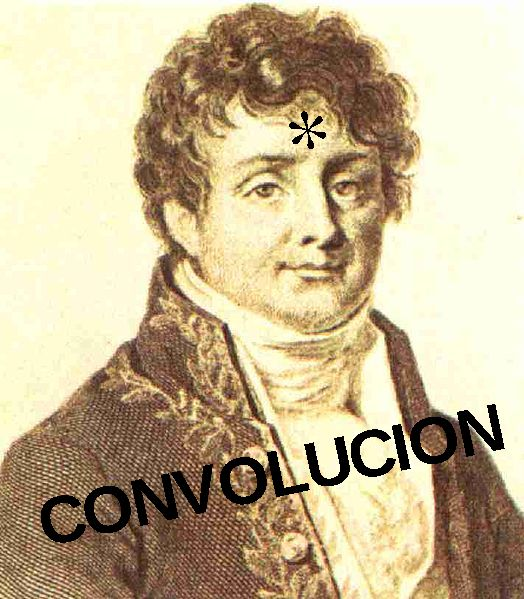
\includegraphics[width=.5\textwidth]{Convolucion}
  \caption{Znani francoski konvolucionar Jean Baptiste Joseph Fourier}
\end{figure}

\section{Konvolucija}

Linearno padajo"co funkcijo $f(x) = 1-x$ sem izvrednostil v $N$ diskretnih to"ckah, nato pa numeri"cno ra"cunal konvolucijo te funkcije samo s sabo. Ta ra"cun sem ponovil pri razli"cnih vrednostih $N$ in ga vsakih napravil na dva na"cina: enkrat po definiciji konvolucije, drugi"c pa z uporabo Fourierove transformacije. Za vse ra"cune sem uporabil program \texttt{GNU Octave}. 

\subsection{Hitrost}

\begin{figure}[h]
 \centering
\input{g_konv_cas}
\caption{"Cas, potreben za izra"cun konvolucije treh linearno padajo"cih funkcij po obeh algoritmih}
\end{figure}

\subsection{Natan"cnost}

Preveril sem tudi, kako natan"cna je metoda s Fourierovo transformacijo. Tako direktna kot FFT metoda ne delata nobenih pribli"zkov, edini vir napake je kon"cna natan"cnost ra"cunalni"skega zapisa, na katerege pa sta lahko metodi razli"cno ob"cutljivi. Kot mero za napako metode sem izbral

\begin{align}
 \sigma^2 &= \sum_{i=0}^{kN-1} (f_i^F - f_i^D)^2
\end{align}

kjer so $f_i^F$ in $f_i^D$ koeficienti, izra"cunani s Fourierovo oz. direktno metodo. "Ce sem za"cel z diskretizacijo na $N$ to"ck in izra"cunal konvolucijo $k$-tih enakih funkcij, ima kon"cni izraz $kN$ koeficientov. 


\begin{figure}[h]
 \centering
\input{g_konv_napaka}
\caption{Napaka izra"cuna s Fourierovo transformacijo}
\end{figure}

\section{Dekonvolucija signala}

Tokrat je bila naloga obratna, poiskati izviren signal ob poznavanju izhodnega signala in prehodne funkcije. Prehodna funkcija $G(t)$ pa je imela en neznani parameter $\beta$, ki sem ga dolocil tako, da je bil izvirni signal "cim lep"si. Lepoto signala pa sem definiral na razli"cne na"cine. 

\begin{figure}[h]
 \input{g_decon_3d}
\end{figure}


\subsection{"Cim manj"se spremembe}

Ena mo"zna izbira je, da i"s"cemo signal, ki se "cim po"casneje spreminja. Naravna izbira je tak"sna, da je izraz

\begin{align}
  \sum_{i=0}^{N-1} \left| s_i - s_{i-1}\right|^2
\end{align}

"cim manj"si. Izka"ze se, da je to pri vrednosti $\beta = 34.852$, vhodni signal pa je tedaj tak kot na sliki~\ref{fig:dekon-signal}. 

\begin{figure}[h]
 \input{g_decon_signal}
\caption{Vhodni in izhodni signal pri $\beta = 34.852$}
\label{fig:dekon-signal}
\end{figure}

\subsection{"Cim ni"zje frekvence}

Lepoto signala pa lahko ocenimo "ze po frekven"cnem spektru, tako da si "zelimo "cim manj visokih frekvenc. V ta namen sem minimiziral izraz

\begin{align}
 \sum_{i=-N/2}^{N/2-1} i\cdot|S_i|
\end{align}

kjer so $S_i$ komponentne Fourierove transformacije signala $s_i$. Ta kriterij je v bistvu zelo podoben prej"snjemu, zato je tudi optimalna vrednost $\beta$ blizu, in sicer $\beta = 36.475$. 

\subsection{"Cim manj"sa amplituda}

Za primerjavo sem iskal tudi signal z najmanj"so amplitudo. "Ce privzamemo, da je signal pribli"zno sinusen, lahko njegovo amplutido ocenimo v vsaki to"cki. 

\begin{align}
 s(t) &= A\sin \omega t \\
 \dot s(t) &= A\omega \cos \omega \\ 
 A^2 &= \omega^2 s^2 + (\dot{s})^2
\end{align}

Odvod $\dot s$ lahko pribli"zamo s kon"cno diferenco, frekven"co $\omega$ pa kot po absolutni vrednosti najve"cjo komponentno Fourierove transformiranke. Seveda na"s signal ni povsem sinusen, zato se amplituda spreminja s "casom, $A = A(t)$. Podobno kot v prvem primeru sem na koncu minimiziral povpre"cen kvadrat amplitude. 

\end{document}
